\documentclass[11pt, a4paper]{article}
%\usepackage{proj1}
\usepackage{natbib}
\usepackage{fancyhdr}  
\usepackage{subcaption}
\usepackage{caption}
\usepackage{graphicx}
\linespread{1.25} 
\setlength{\parindent}{0cm}
\graphicspath{{Images/}}
\usepackage{hyperref}
\usepackage{amsmath}
\usepackage{amsfonts}
\usepackage{amssymb}
\usepackage{amsthm}
\usepackage{mathtools}
\usepackage{commath}
\usepackage[warning,debug,nosepfour,autolanguage]{numprint}

%\usepackage[sc,osf]{mathpazo}
\usepackage{subcaption}
\usepackage[a4paper, top=1in, left=1.0in, right=1.0in, bottom=1in, includehead, includefoot]{geometry} %Usually have top as 1in

\usepackage{listings}
\usepackage{color} %red, green, blue, yellow, cyan, magenta, black, white
\definecolor{mygreen}{RGB}{28,172,0} % color values Red, Green, Blue
\definecolor{mylilas}{RGB}{170,55,241}


\hypersetup{colorlinks,linkcolor={black},citecolor={blue},urlcolor={black}}
\usepackage{color}
\urlstyle{same}


\theoremstyle{definition}
\newtheorem{definition}{Definition}[section]

\title{Exact Solutions for the Full Problem \\with Force Control and with Flow Control}
\date{}
\newcommand{\Sta}{\rho}
\newcommand{\Adj}{p}
\newcommand{\Con}{u}

\pagenumbering{gobble}
\begin{document}
	
\begin{table}
	\begin{tabular}{ ||c|| c | c |c | c ||}
		gamma & beta & Iters  & JFW & JOpt \\
		$\numprint{1e-03}$ & $\numprint{ 0.000 }$ & $\numprint{ 671 }$ & $\numprint{ 0.04166667 }$ & $\numprint{ 0.00144668 }$ \\
		$\numprint{1e-03}$ & $\numprint{ 0.000 }$ & $\numprint{ 726 }$ & $\numprint{ 0.06690197 }$ & $\numprint{ 0.01091870 }$ \\
	\end{tabular}
\end{table}
	
	Notes/ Questions on Report:\\
	- Paper plots: color bar from t0 to T or other way around?\\
	- don't know what's up with this extra arrow in the vector plots.\\
	- Comment: Figure 8 to 11 and Figure 14 to 17 are the interesting examples.\\
	Currently running some configurations of Ex2 and Ex4 on server.\\
	Notes/ Questions on Presentation:\\
	- only Neumann Flow control below.\\
	- summary slide: different models?\\
	- how to call $\vec{w}$ in talk (I'll explain what I mean by this).\\
	- if too long, what should go?\\
	- figure references ok?

\section{Paper plots fixed}
See figures \ref{PPPL1}, \ref{PPPL2} and \ref{PPPL3}.
\begin{figure}[h]
	\includegraphics[scale=0.3]{PPPL1.png}
	\caption{Example 1.}
	\label{PPPL1}
\end{figure}
\begin{figure}[h]
	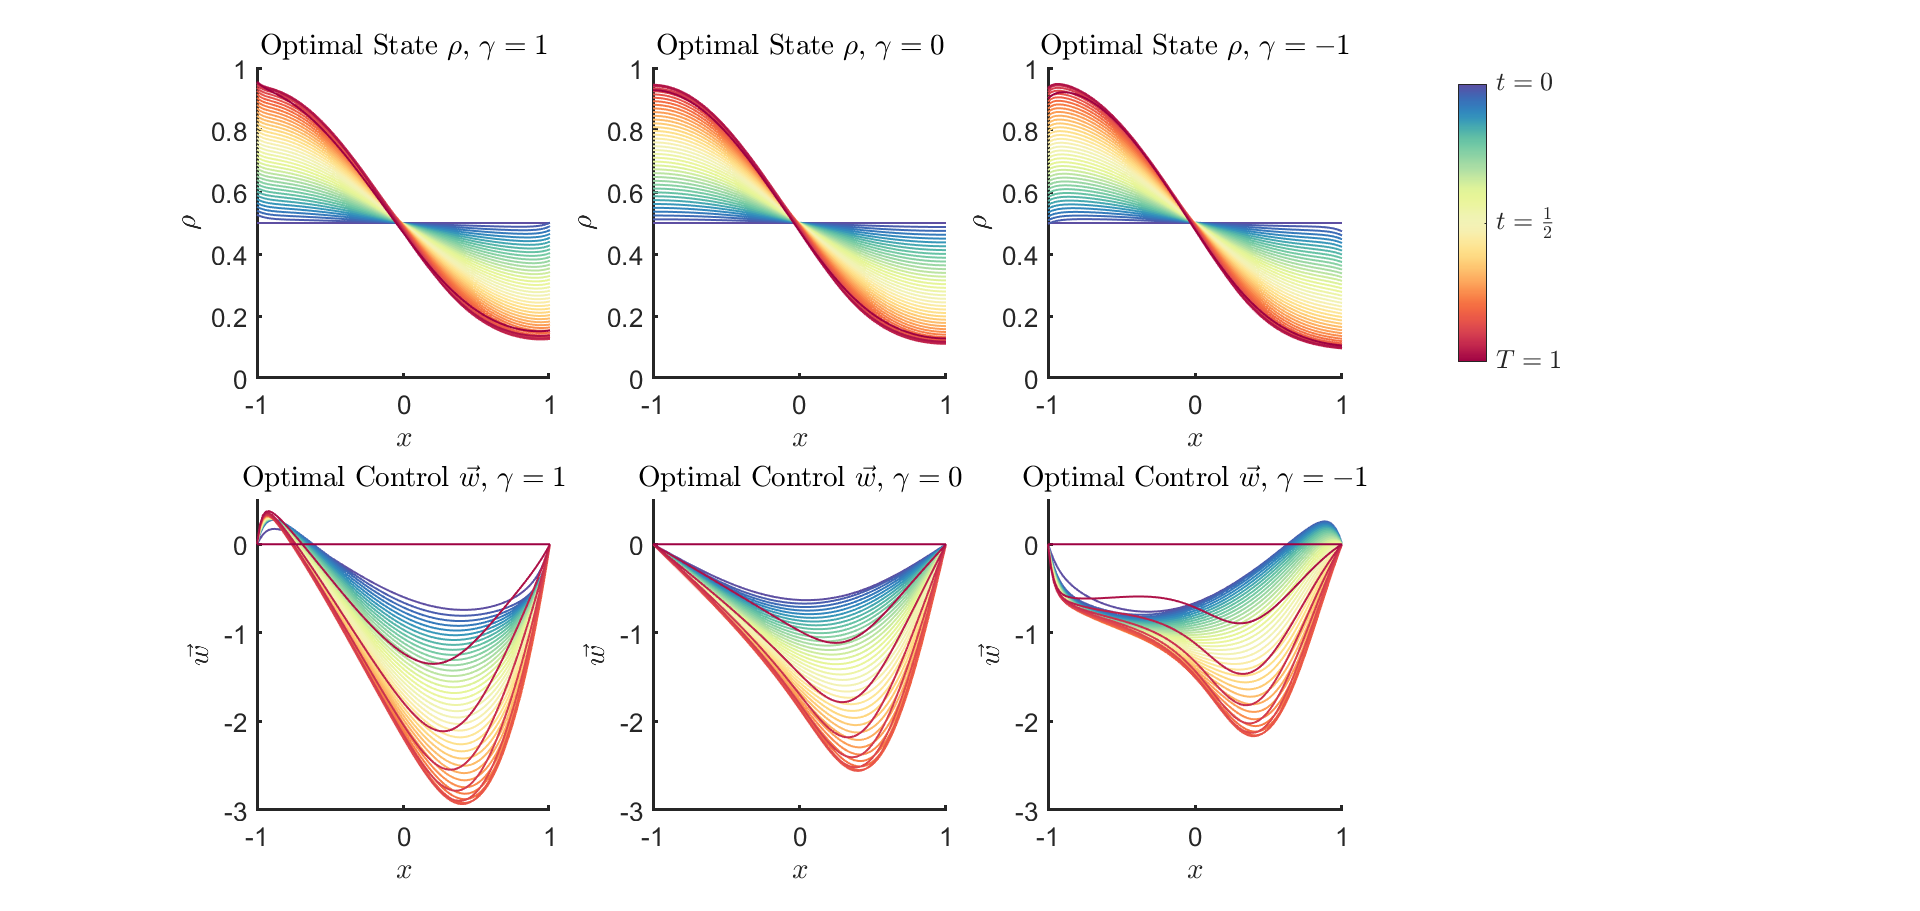
\includegraphics[scale=0.3]{PPPL2.png}
	\caption{Example 1.}
	\label{PPPL2}
\end{figure}
\begin{figure}[h]
	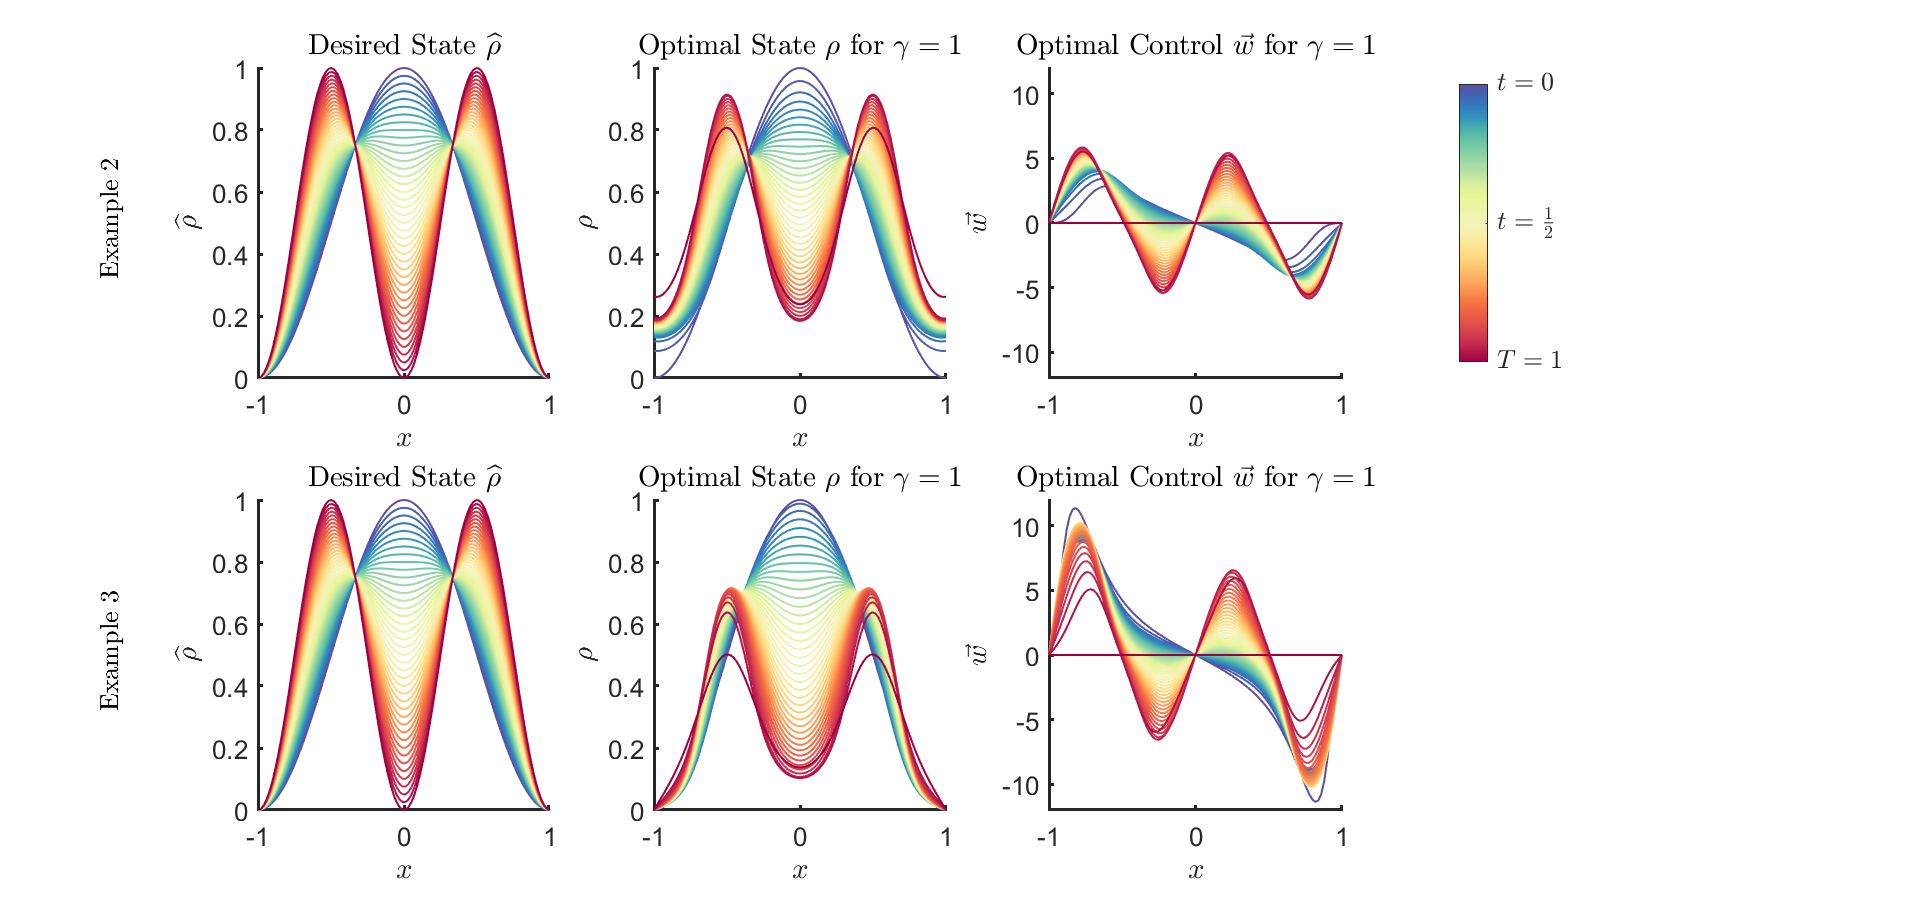
\includegraphics[scale=0.3]{PPPL3.png}
	\caption{Example 2/ Example 3.}
	\label{PPPL3}
\end{figure}
\section{2D Example 1}
We choose $\rho_0 = 0.25$ and
\begin{align*}
\hat \rho = 0.25(1-t) + t\frac{1}{4}((\cos(\pi y_1)+1)(\cos(\pi y_2)+1)),  
\end{align*}
as in last week's report. See figures \ref{rhoHat2d1a} and \ref{rhoOpt2d1a}.
\begin{figure}[h]
	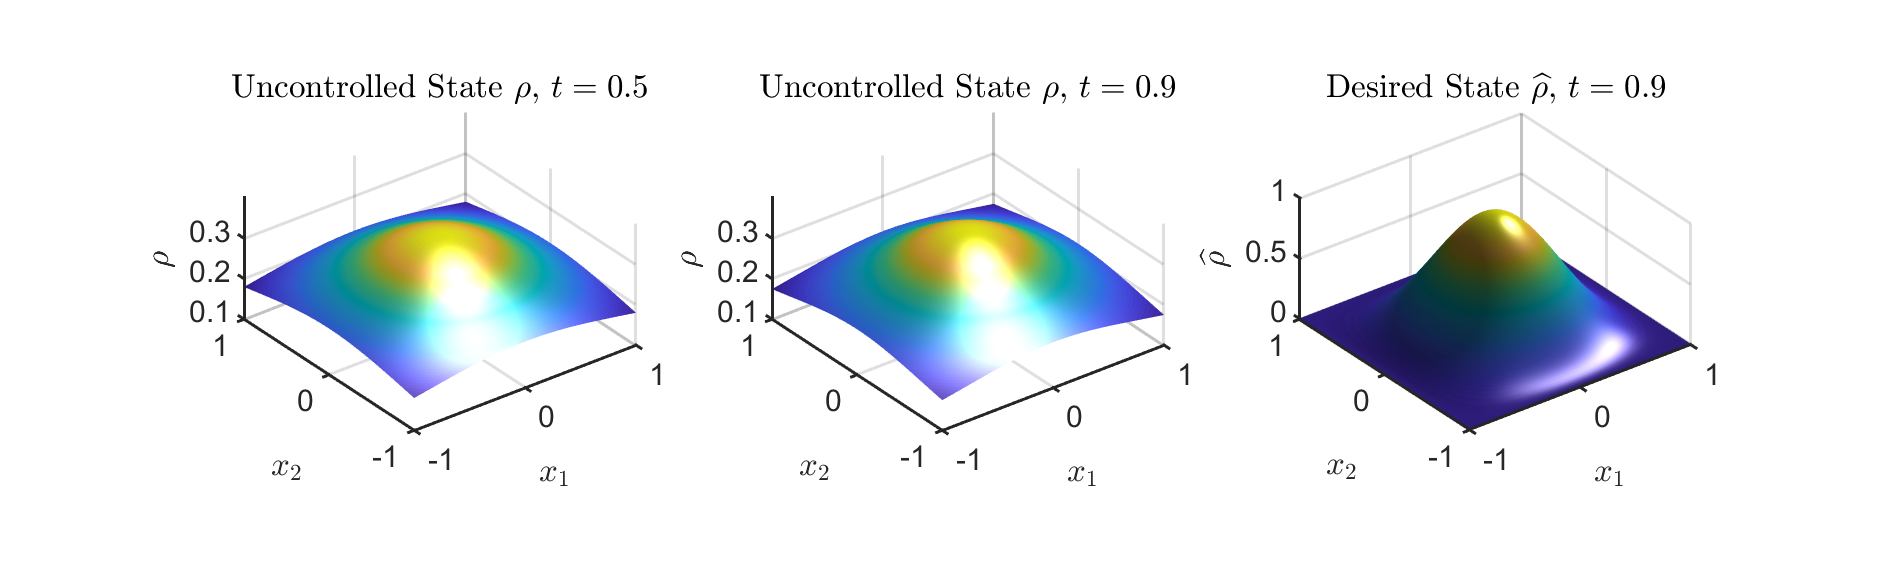
\includegraphics[scale=0.3]{Res1a.png}
	\caption{2D Example 1, uncontrolled $\rho$ and $\widehat \rho$, $\beta = 10^{-3}$, $\gamma = -1$.}
	\label{rhoHat2d1a}
\end{figure}
\begin{figure}[h]
	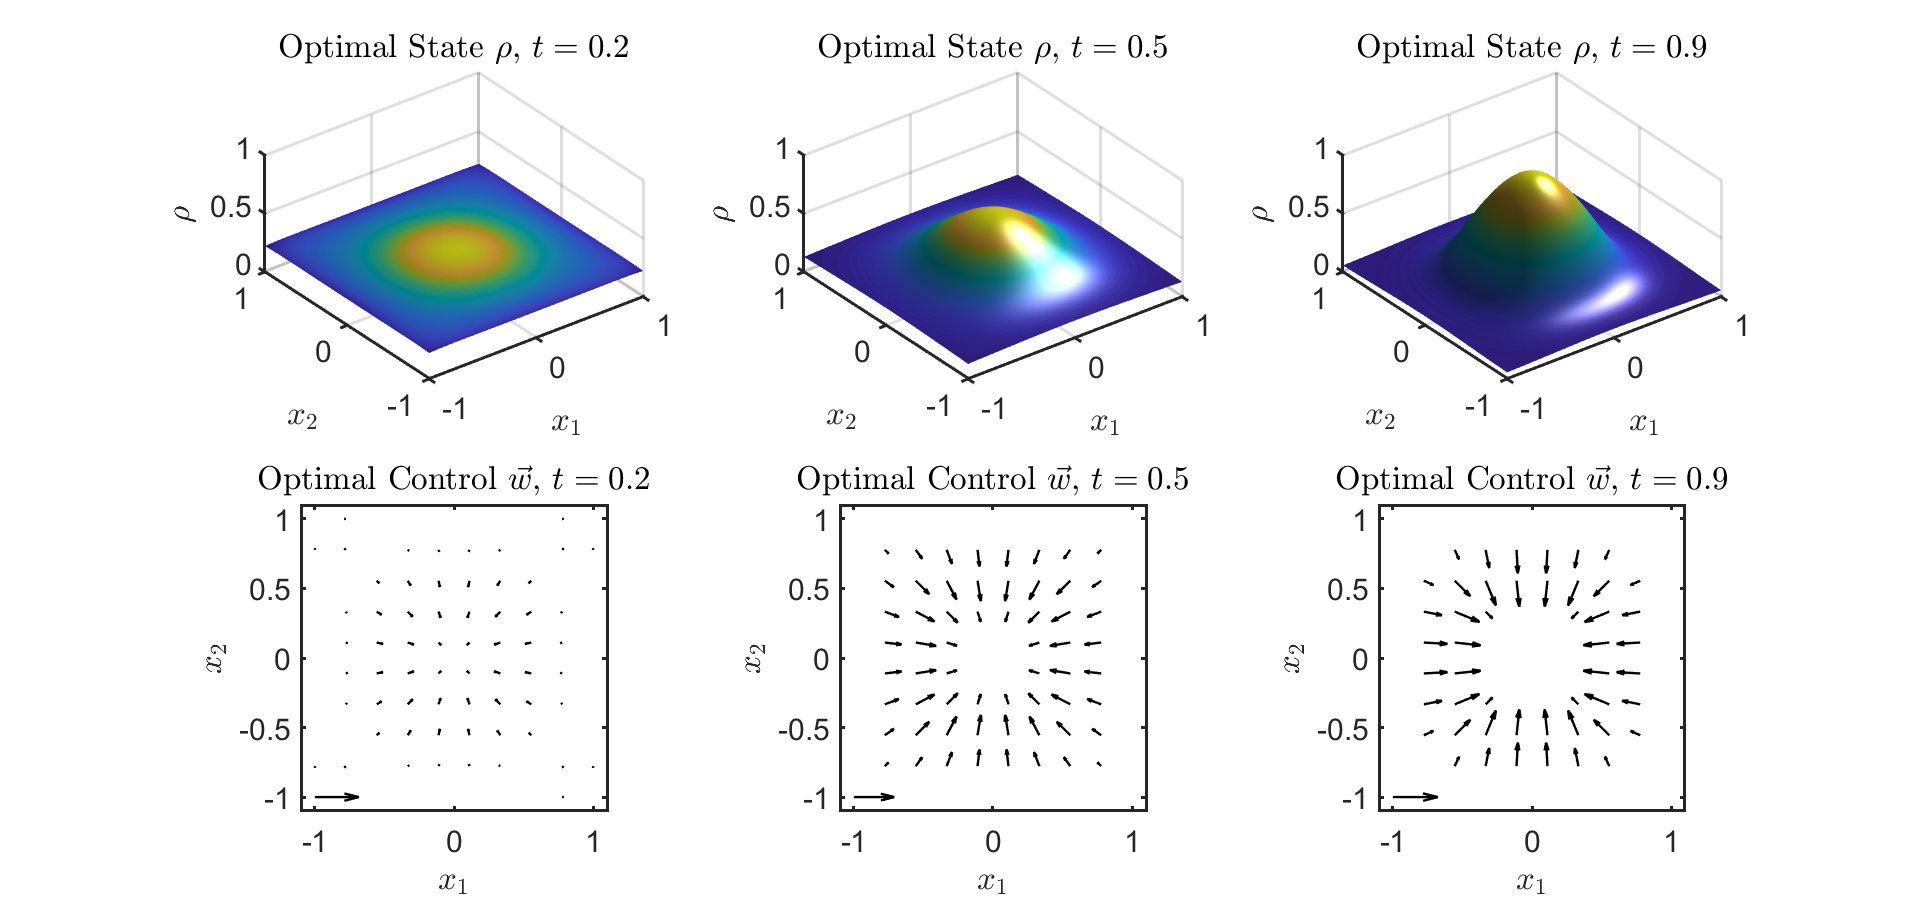
\includegraphics[scale=0.3]{Res2a.png}
	\caption{2D Example 1, controlled $\rho$ and optimal control $\vec{w}$, $\beta = 10^{-3}$, $\gamma = -1$.}
	\label{rhoOpt2d1a}
\end{figure}
\begin{figure}[h]
	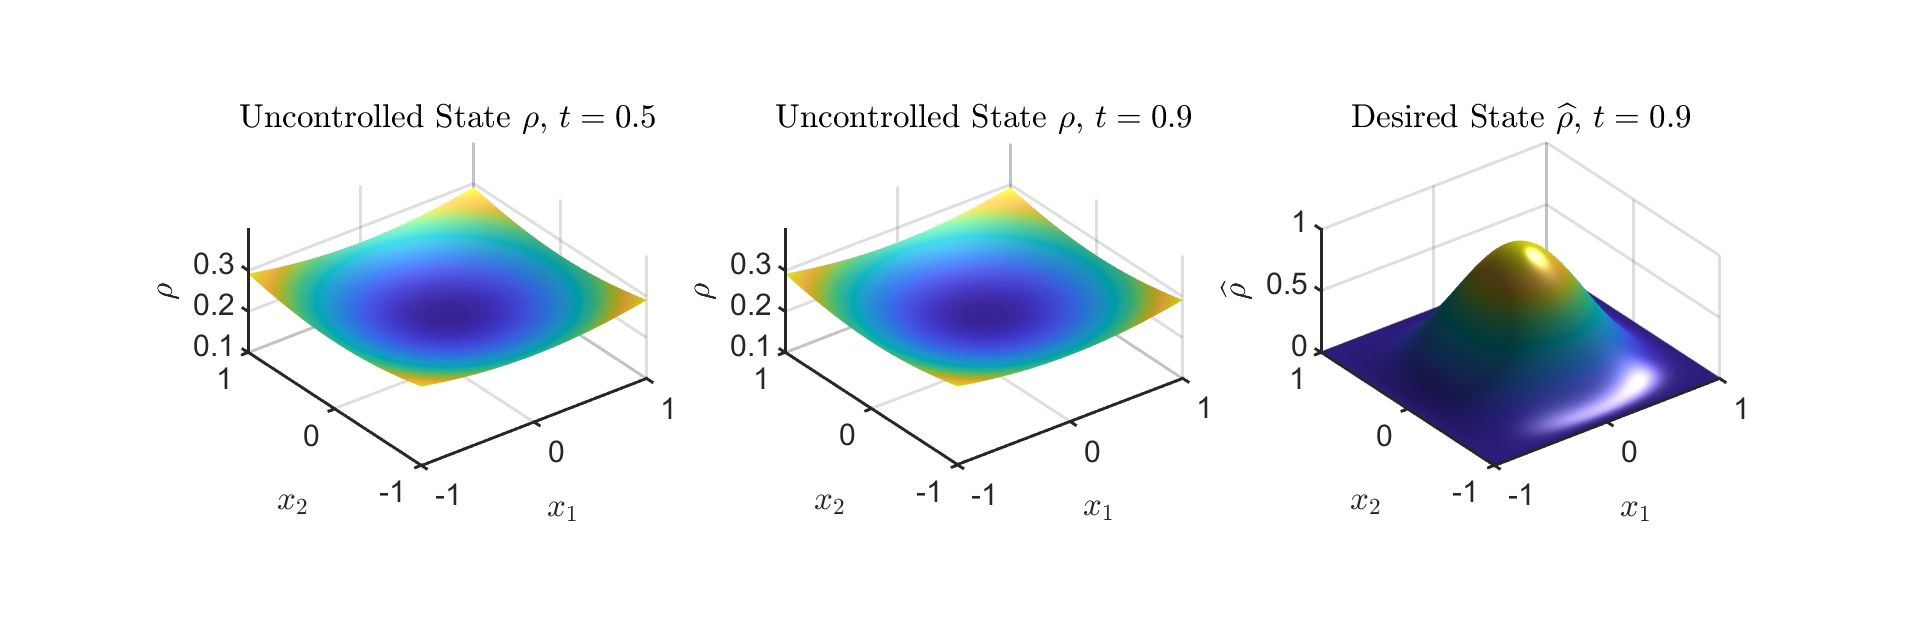
\includegraphics[scale=0.3]{Res1b.png}
	\caption{2D Example 1, uncontrolled $\rho$ and $\widehat \rho$, $\beta = 10^{-3}$, $\gamma = 1$.}
	\label{rhoHat2d1b}
\end{figure}
\begin{figure}[h]
	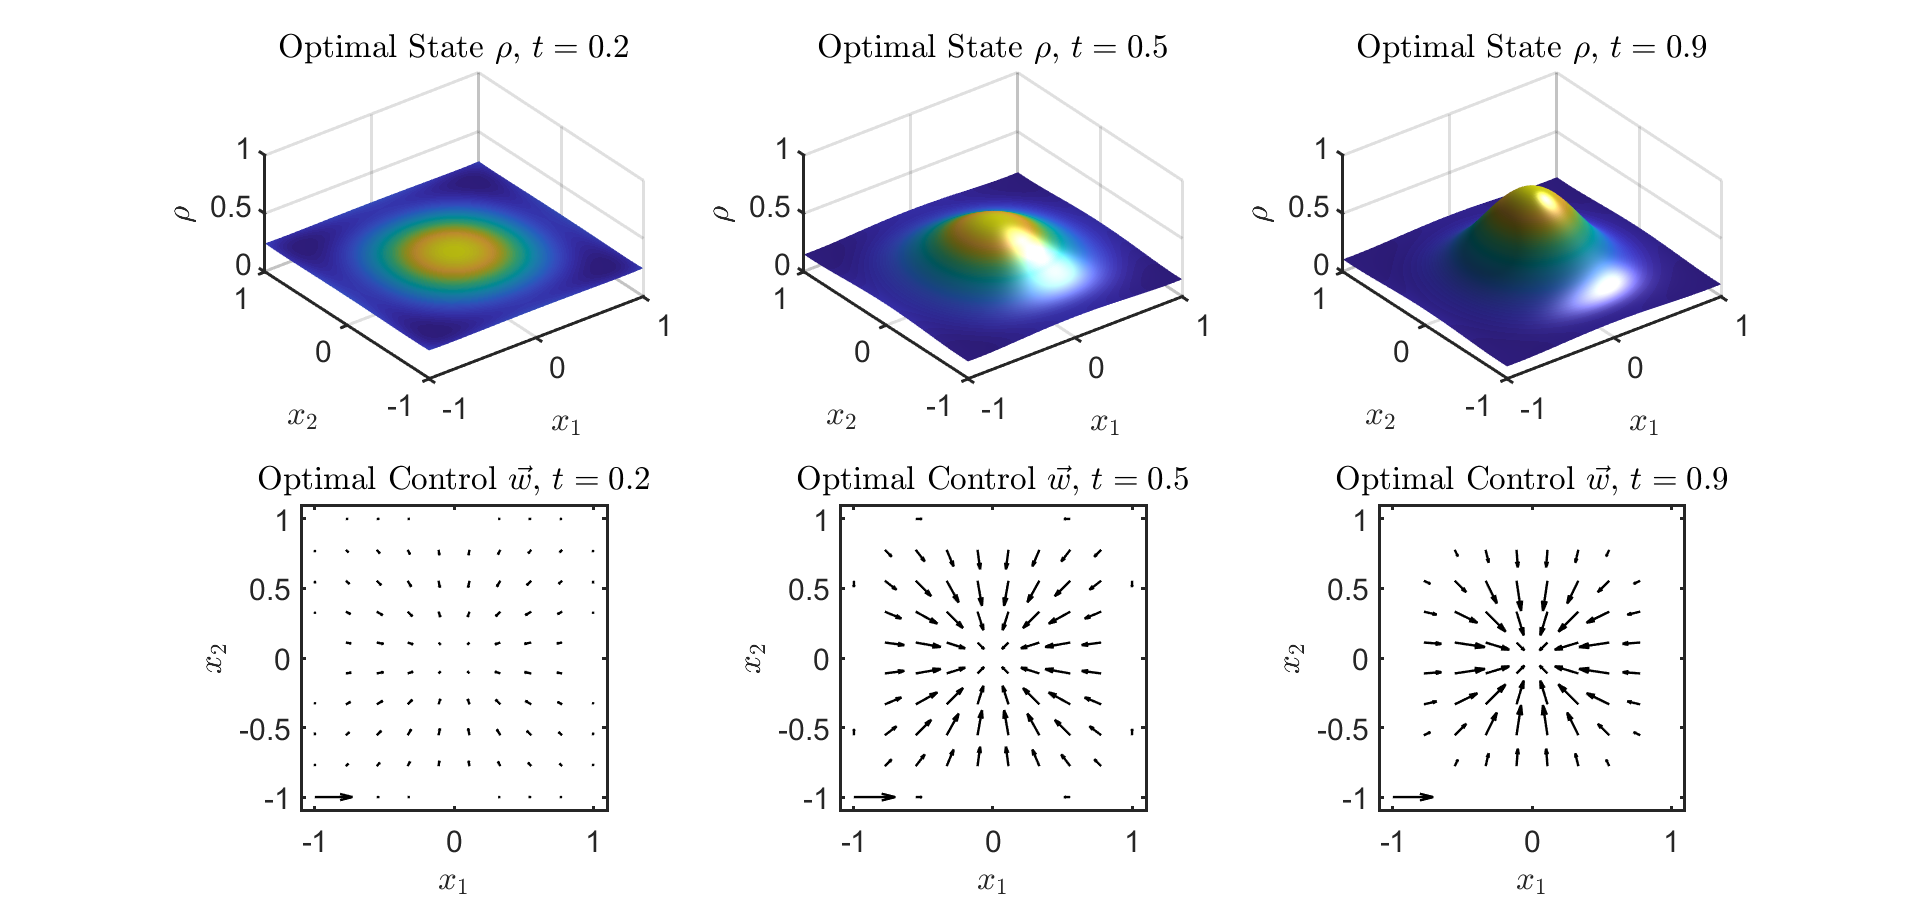
\includegraphics[scale=0.3]{Res2b.png}
	\caption{2D Example 1, controlled $\rho$ and optimal control $\vec{w}$, $\beta = 10^{-3}$, $\gamma = 1$.}
	\label{rhoOpt2d1b}
\end{figure}

\section{2D Example 2}
Choose $\rho_0 = 0.25$ and target:
\begin{align*}
\widehat \rho = \frac{1}{4}(1-t) + t\bigg(\frac{1}{4}\sin \bigg(\frac{\pi}{2}(x_1 - 2)\bigg)\sin \bigg(\frac{\pi}{2}(x_2 - 2)\bigg) + \frac{1}{4}\bigg).
\end{align*}

Choose $n = 10$, $N = 20$ (probably need more in the future but it's quick).
For $\beta = 10^{-3}$, $\gamma = -1$, we get $J_{FW} = 0.0130$ and $J_{Opt} = 7.2994 \times 10^{-4}$, see figures \ref{rhoHat2dEx2} and \ref{rhoOpt2dEx2}.
\begin{figure}[h]
	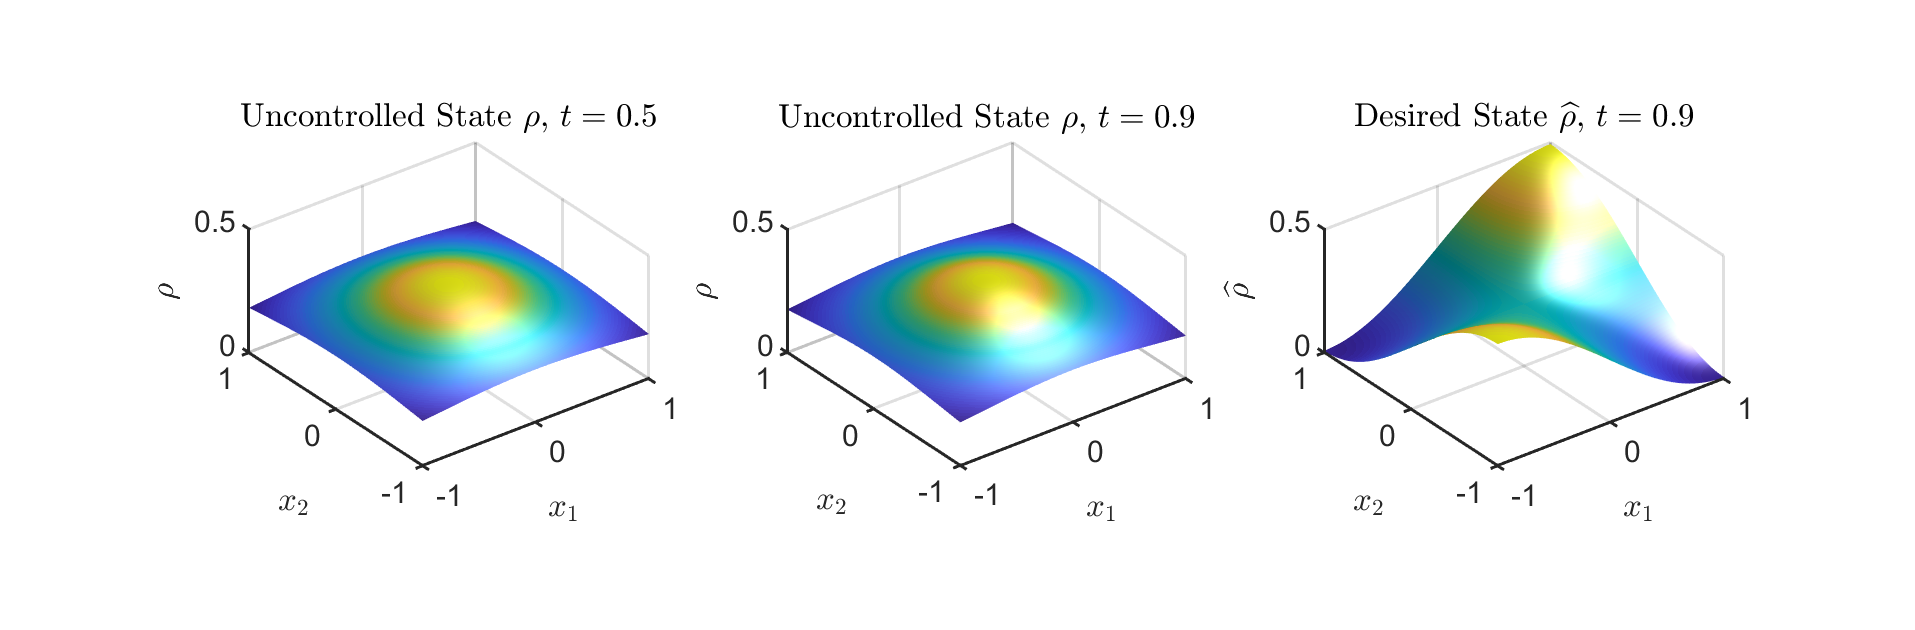
\includegraphics[scale=0.3]{Res1Ex2.png}
	\caption{2D Example 2, uncontrolled $\rho$ and $\widehat \rho$, $\beta = 10^{-3}$, $\gamma = -1$.}
	\label{rhoHat2dEx2}
\end{figure}
\begin{figure}[h]
	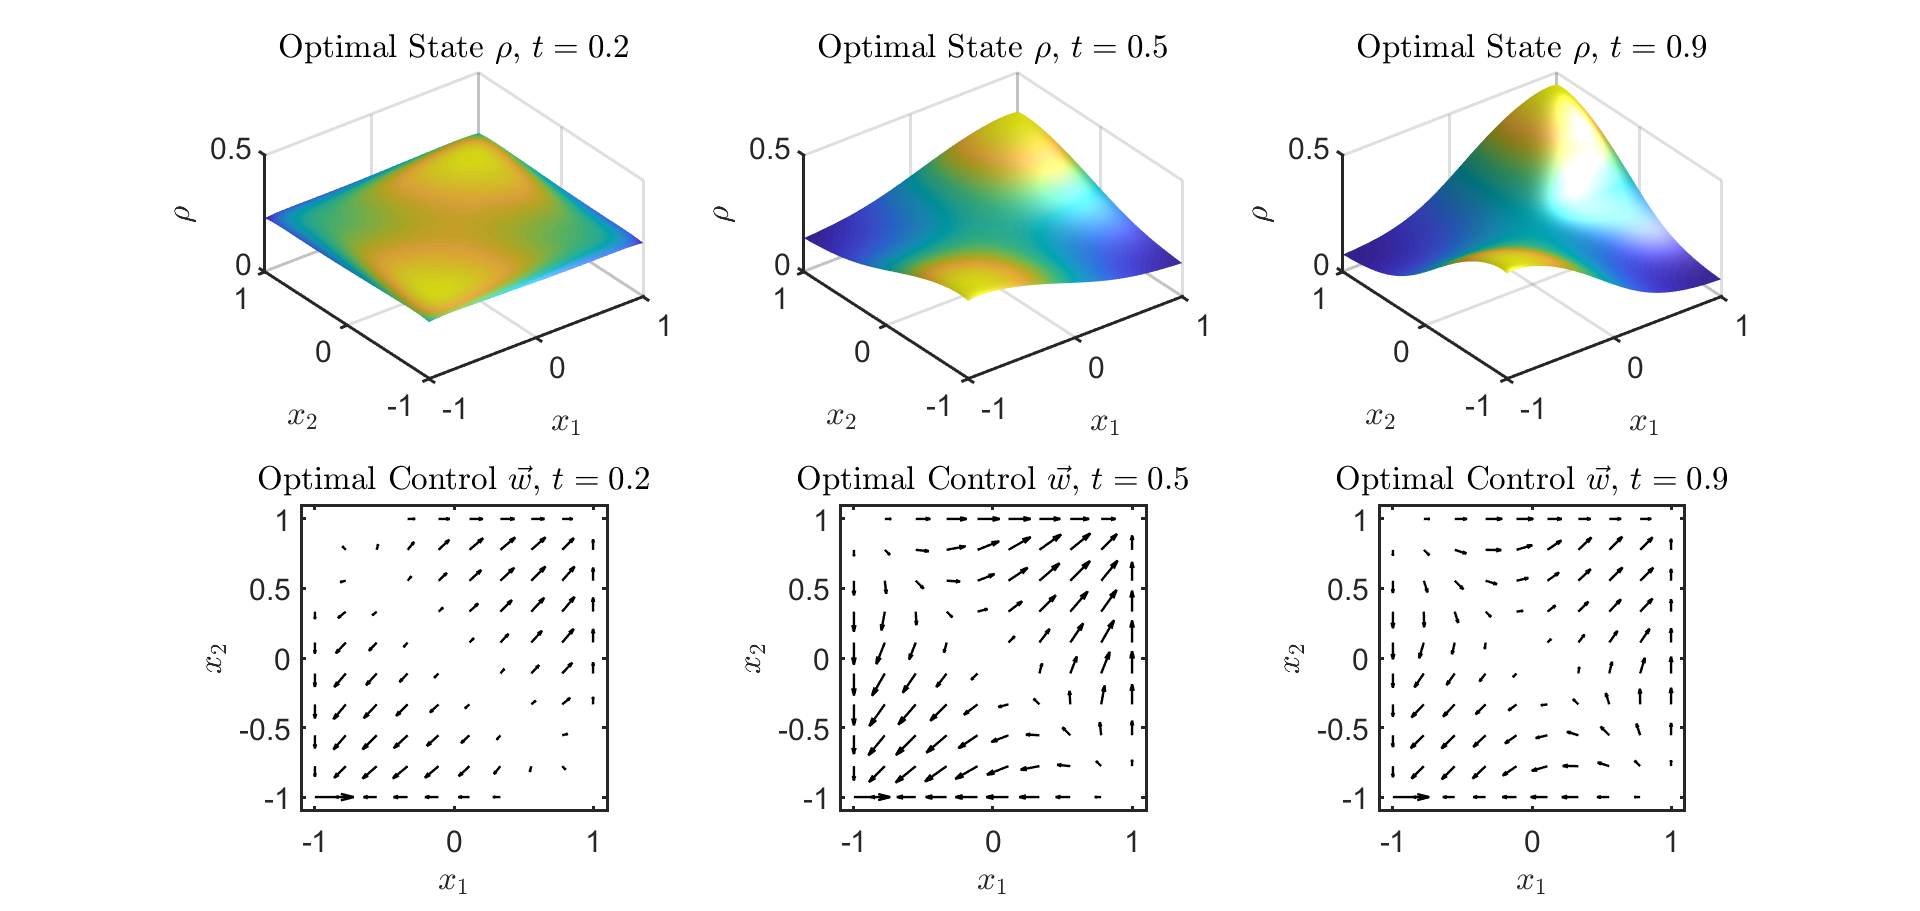
\includegraphics[scale=0.3]{Res2Ex2.png}
	\caption{2D Example 2, controlled $\rho$ and optimal control $\vec{w}$, $\beta = 10^{-3}$, $\gamma = -1$.}
	\label{rhoOpt2dEx2}
\end{figure}
For $\beta = 10^{-3}$, $\gamma = 1$, we get $J_{FW} = 0.0108$ and $J_{Opt} = 0.0023$, see figures \ref{rhoHat2dEx2a} and \ref{rhoOpt2dEx2a}.
\begin{figure}[h]
	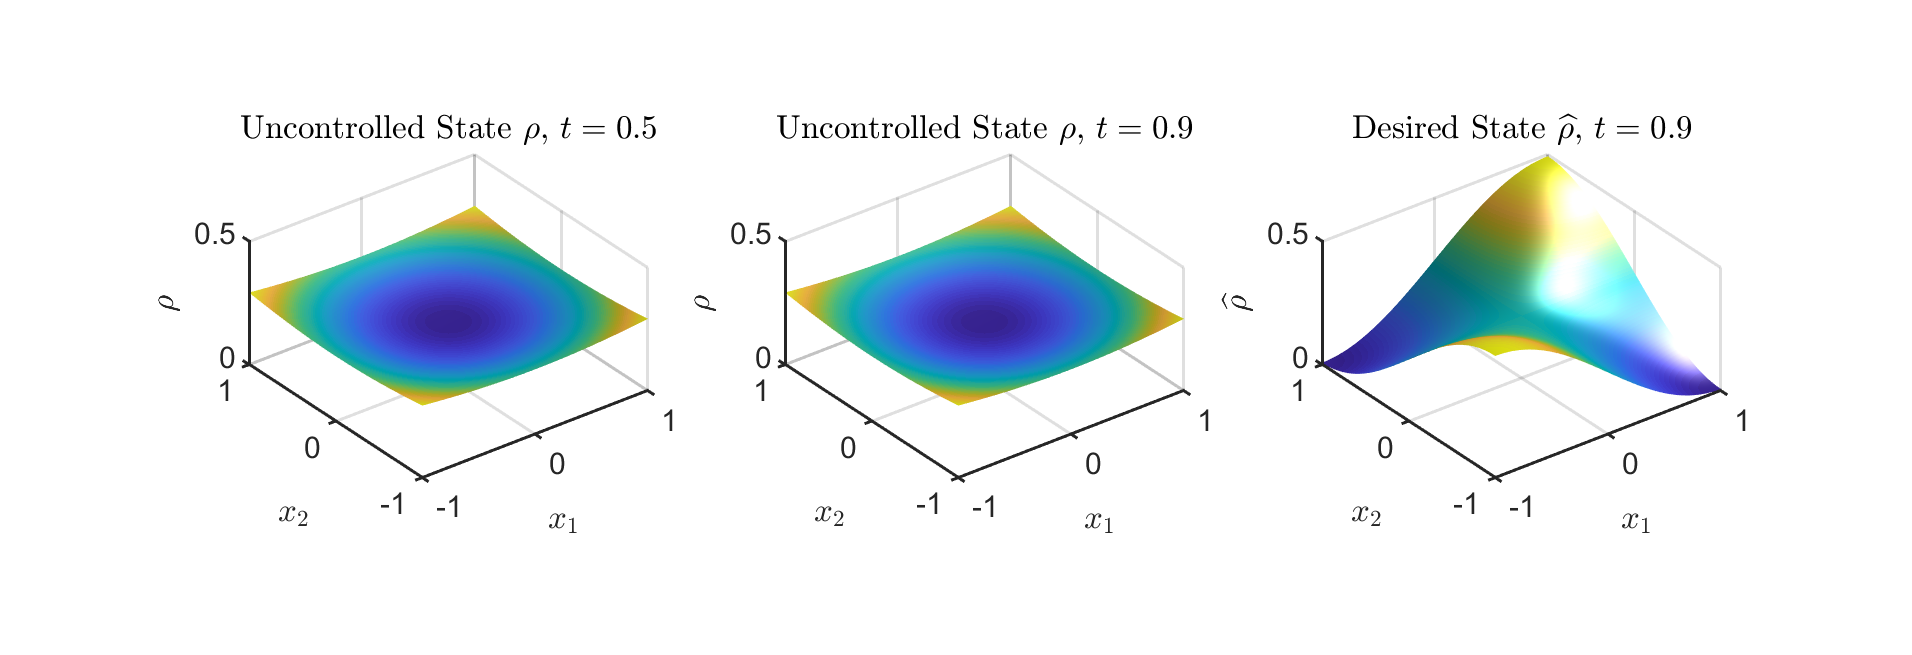
\includegraphics[scale=0.3]{Res1Ex2a.png}
	\caption{2D Example 2, uncontrolled $\rho$ and $\widehat \rho$, $\beta = 10^{-3}$, $\gamma = 1$.}
	\label{rhoHat2dEx2a}
\end{figure}
\begin{figure}[h]
	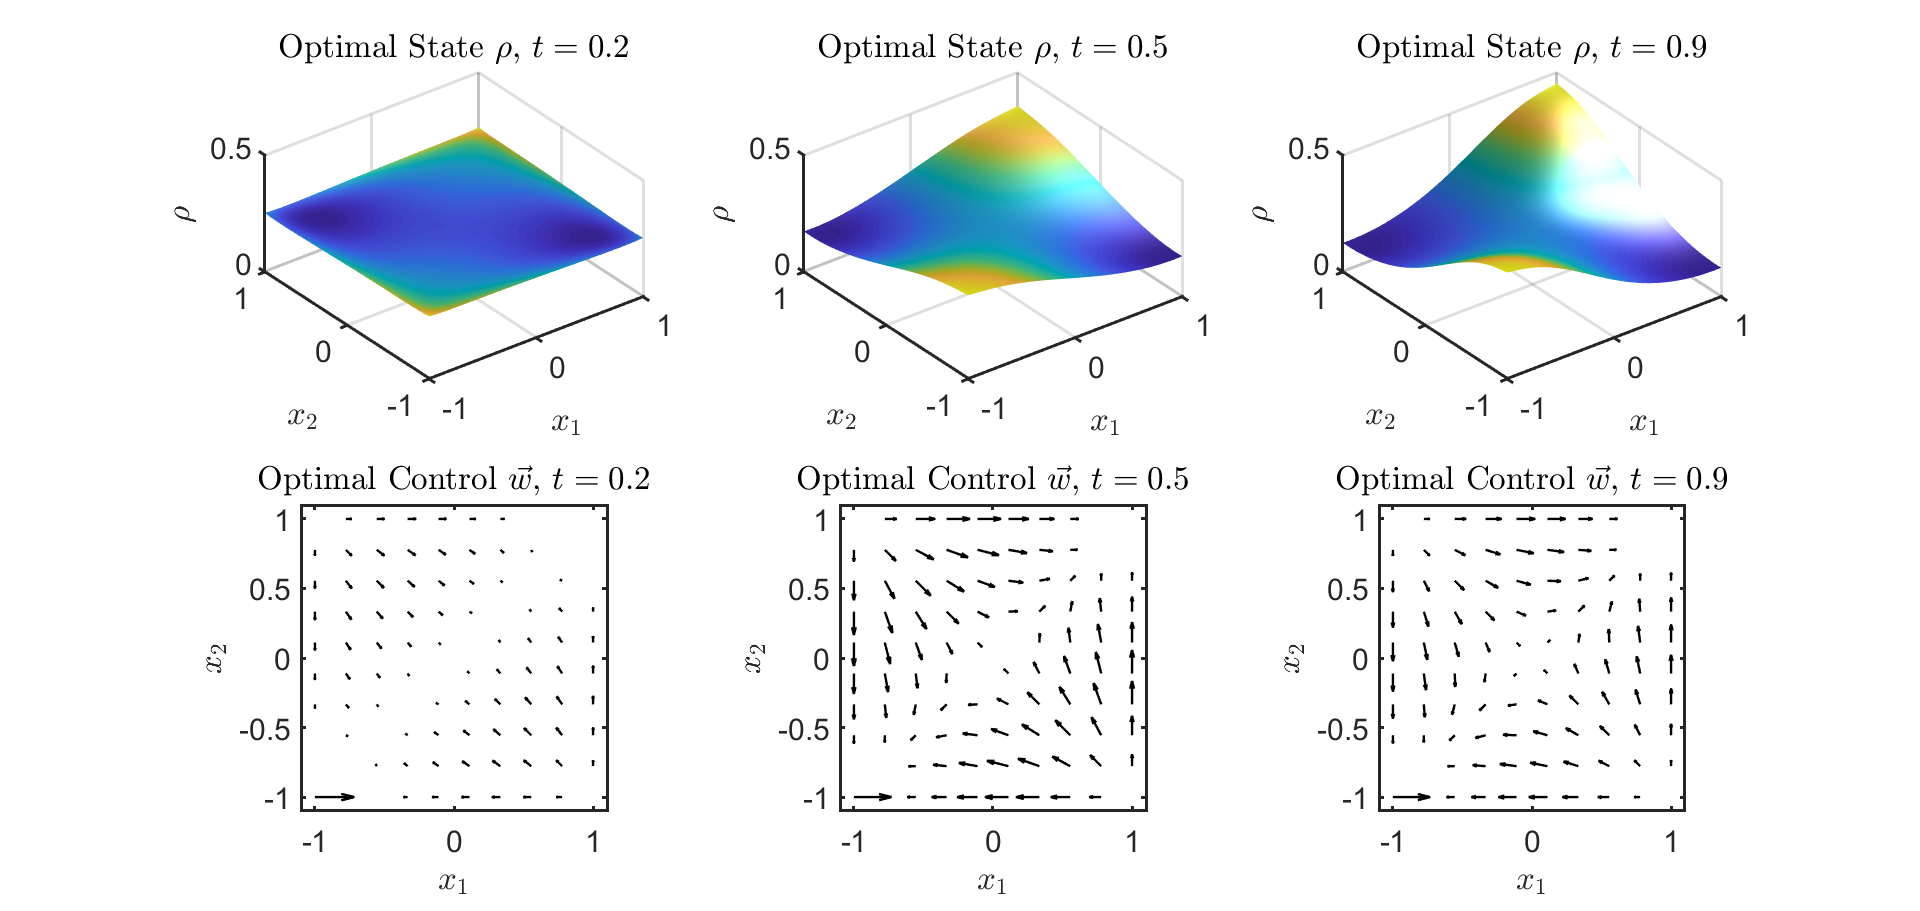
\includegraphics[scale=0.3]{Res2Ex2a.png}
	\caption{2D Example 2, controlled $\rho$ and optimal control $\vec{w}$, $\beta = 10^{-3}$, $\gamma = 1$.}
	\label{rhoOpt2dEx2a}
\end{figure}
	
\section{2D Example 3}
Choose $\rho_0 = \frac{1}{4}$ and the target:
\begin{align*}
\widehat \rho = \frac{1}{4}(1-t) + t\frac{1}{0.31405}e^{-10((y_1+0.2)^2 + (y_2+0.2)^2))}.
\end{align*}
Note the target doesn't satisfy the boundary conditions.	
This converges for $\beta = 10^{-1}$ but diverges for $\beta = 10^{-3}$ for various $N,n$ and $\gamma$. Probably due to steep $\widehat \rho$, so for small $\beta$ we have advection dominance.
Choose $\beta = 10^{-1}$, $n =20$, $N=30$, Tols $= 10^{-8}/10^{-4}$. Then for $\gamma = -1$, we get $J_{FW} = 0.1993$, $J_{Opt} = 0.1595$, see figures \ref{rhoHat2d1} and \ref{rhoOpt2d1}.
\begin{figure}[h]
	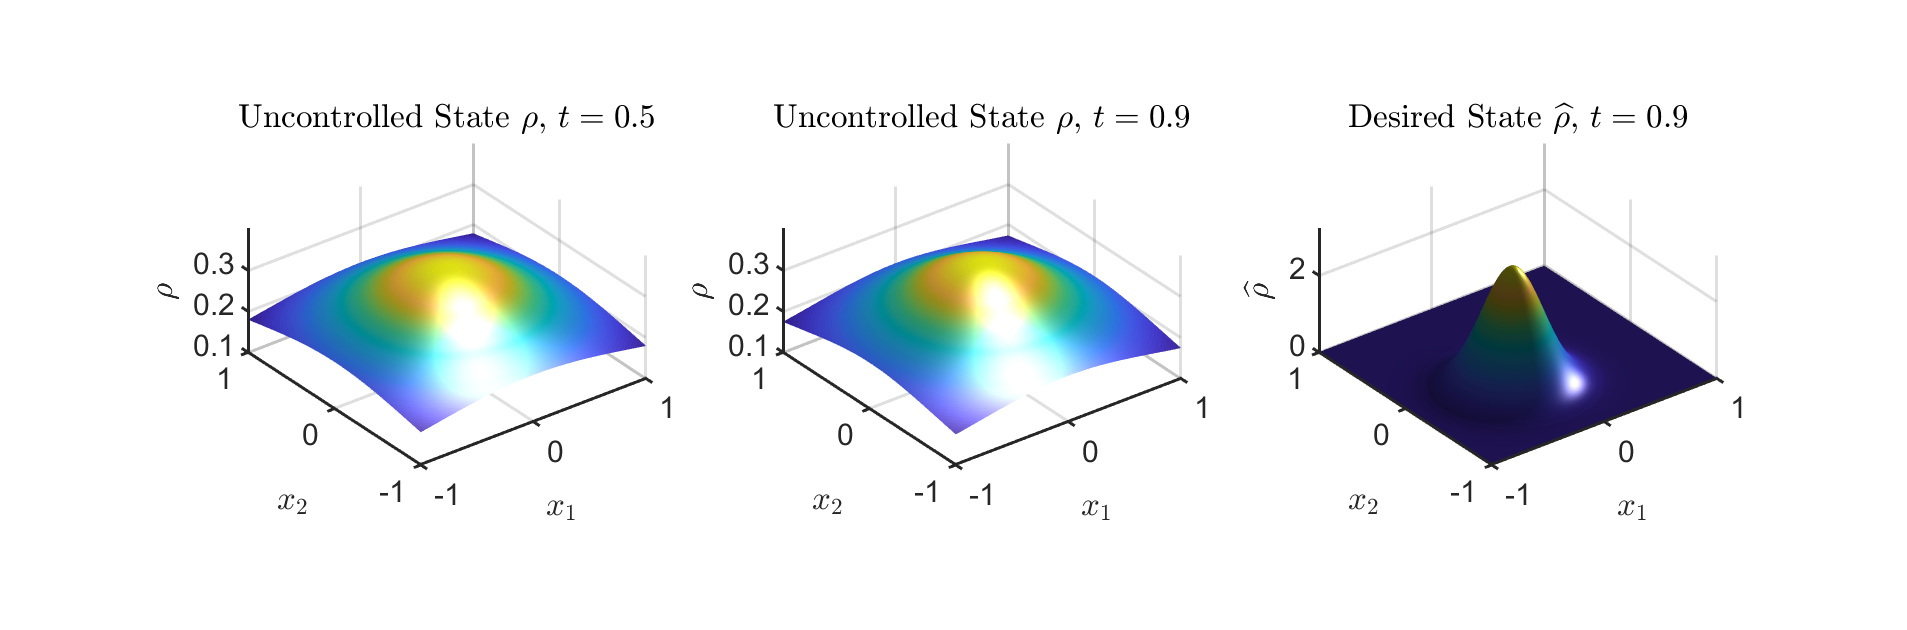
\includegraphics[scale=0.3]{Res1.png}
	\caption{2D Example 3, uncontrolled $\rho$ and $\widehat \rho$, $\beta = 10^{-1}$, $\gamma = -1$.}
	\label{rhoHat2d1}
\end{figure}
\begin{figure}[h]
	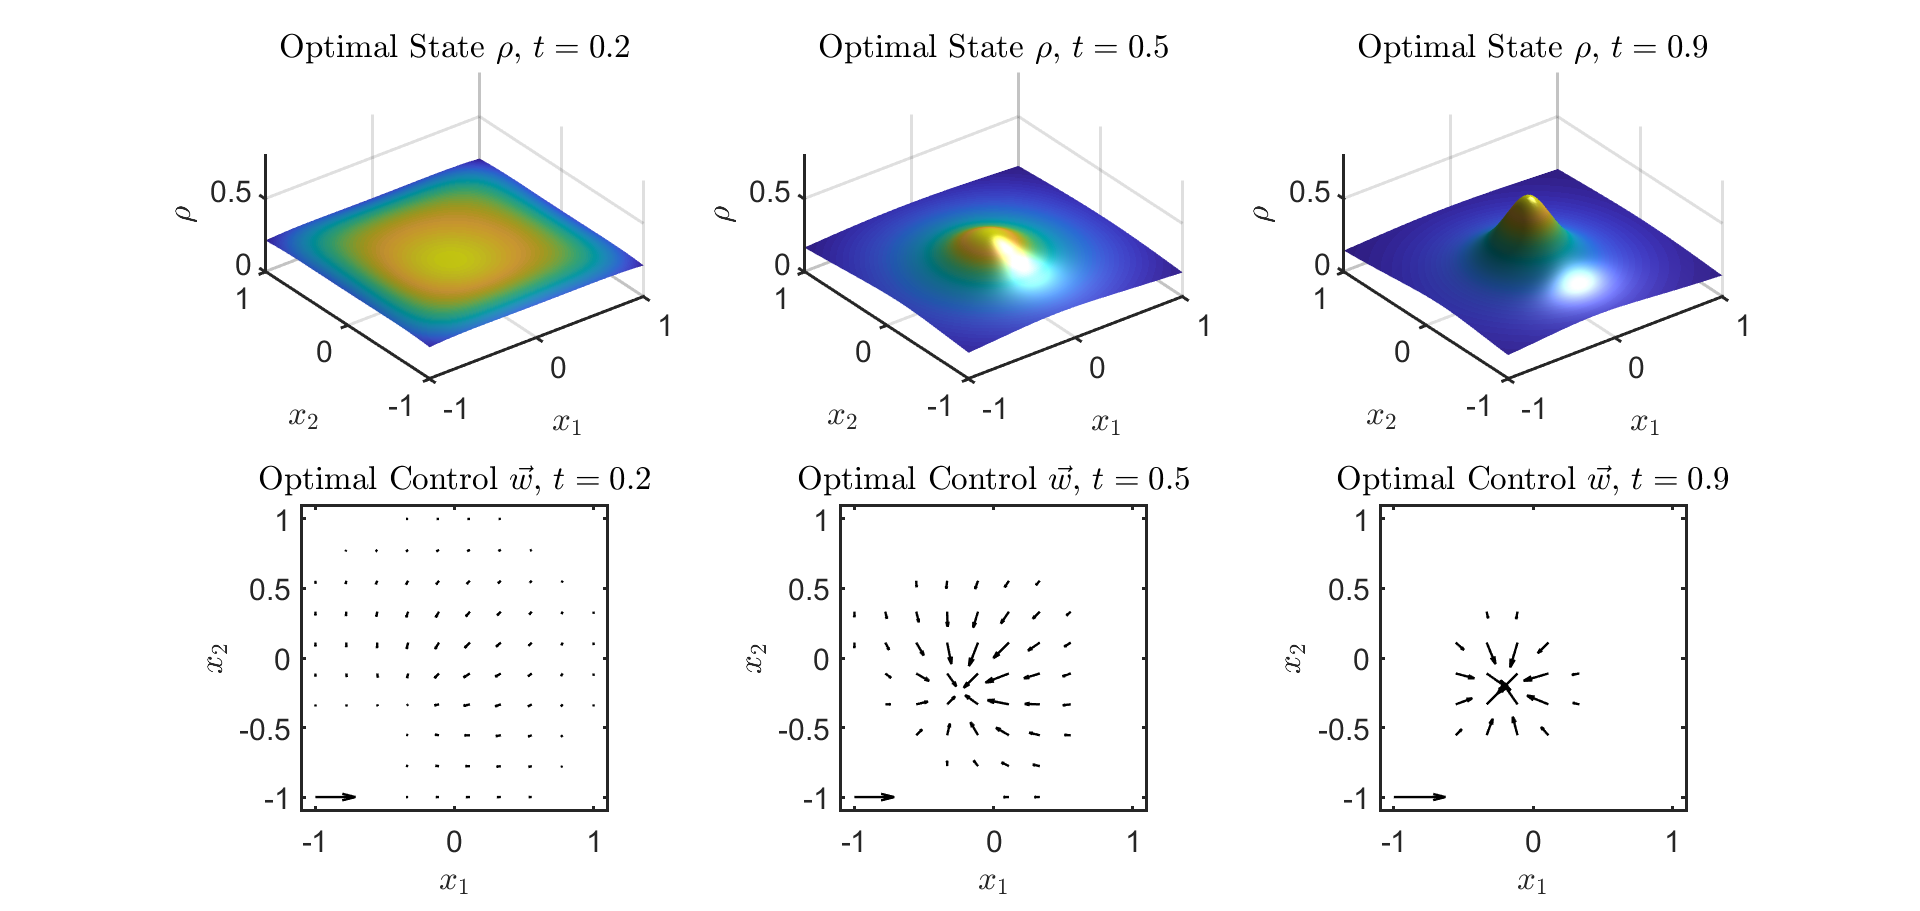
\includegraphics[scale=0.3]{Res2.png}
	\caption{2D Example 3, controlled $\rho$ and optimal control $\vec{w}$, $\beta = 10^{-1}$, $\gamma = -1$.}
	\label{rhoOpt2d1}
\end{figure}	

	
\section{2D Example 4}
We consider a very similar example to Example 3, but with less steep desired state.
We have $\rho_0 = 0.25$, as before, and the target:
\begin{align*}
\widehat \rho = \frac{1}{4}(1-t) + t\frac{1}{0.9921}e^{-3((y_1+0.2)^2 + (y_2+0.2)^2))}.
\end{align*}
Again, this does not satisfy the no-flux boundary conditions.
We have $n=10$, $N=20$, which needs to be increased in the future. 

Then for $\gamma = -1$, we get $J_{FW} = 0.0329$, $J_{Opt} = 0.0014$, see figures \ref{rhoHat2dEx4} and \ref{rhoOpt2dEx4}.
\begin{figure}[h]
	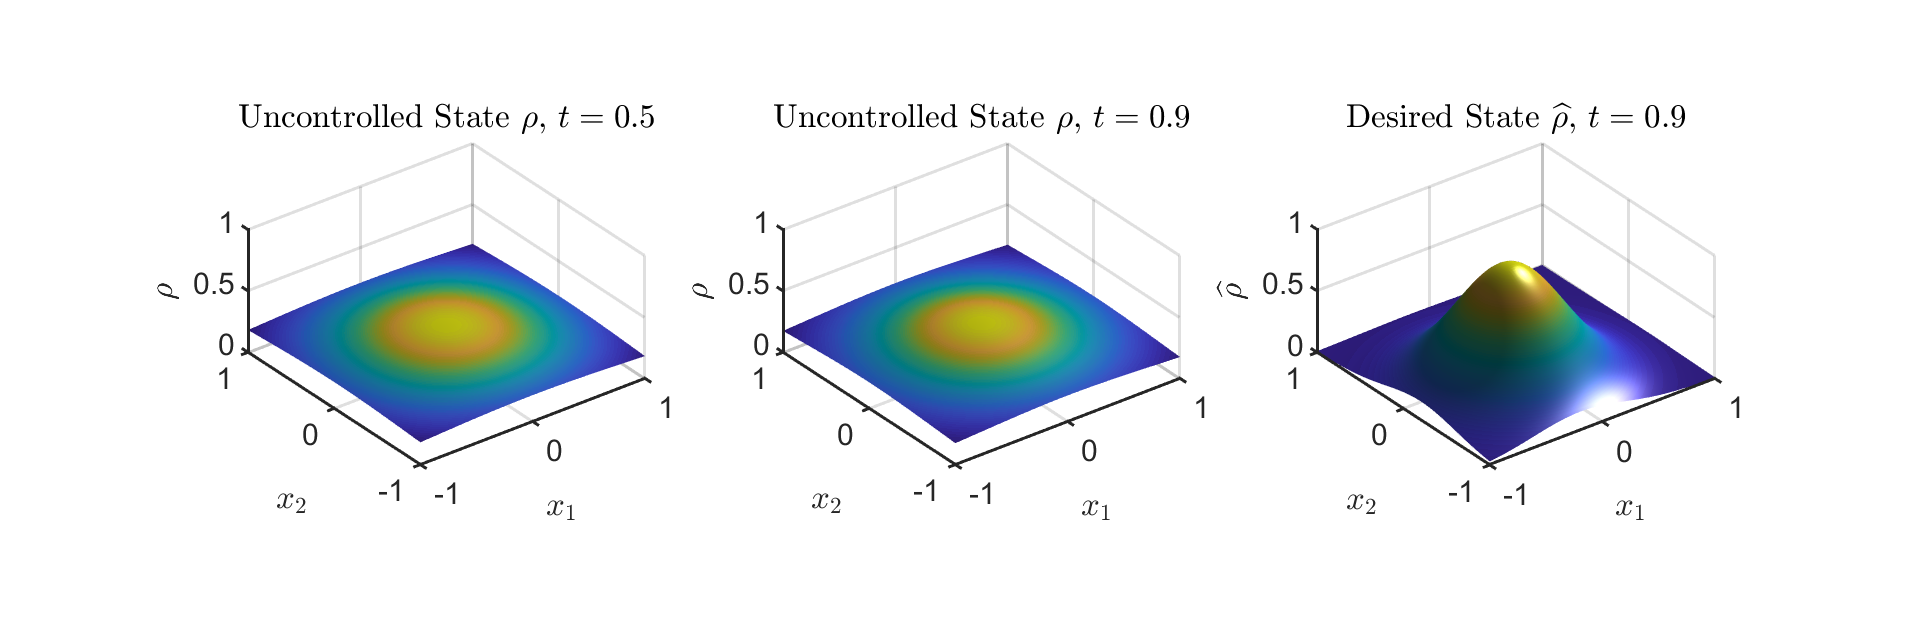
\includegraphics[scale=0.3]{Res1Ex4.png}
	\caption{2D Example 4, uncontrolled $\rho$ and $\widehat \rho$, $\beta = 10^{-3}$, $\gamma = -1$.}
	\label{rhoHat2dEx4}
\end{figure}
\begin{figure}[h]
	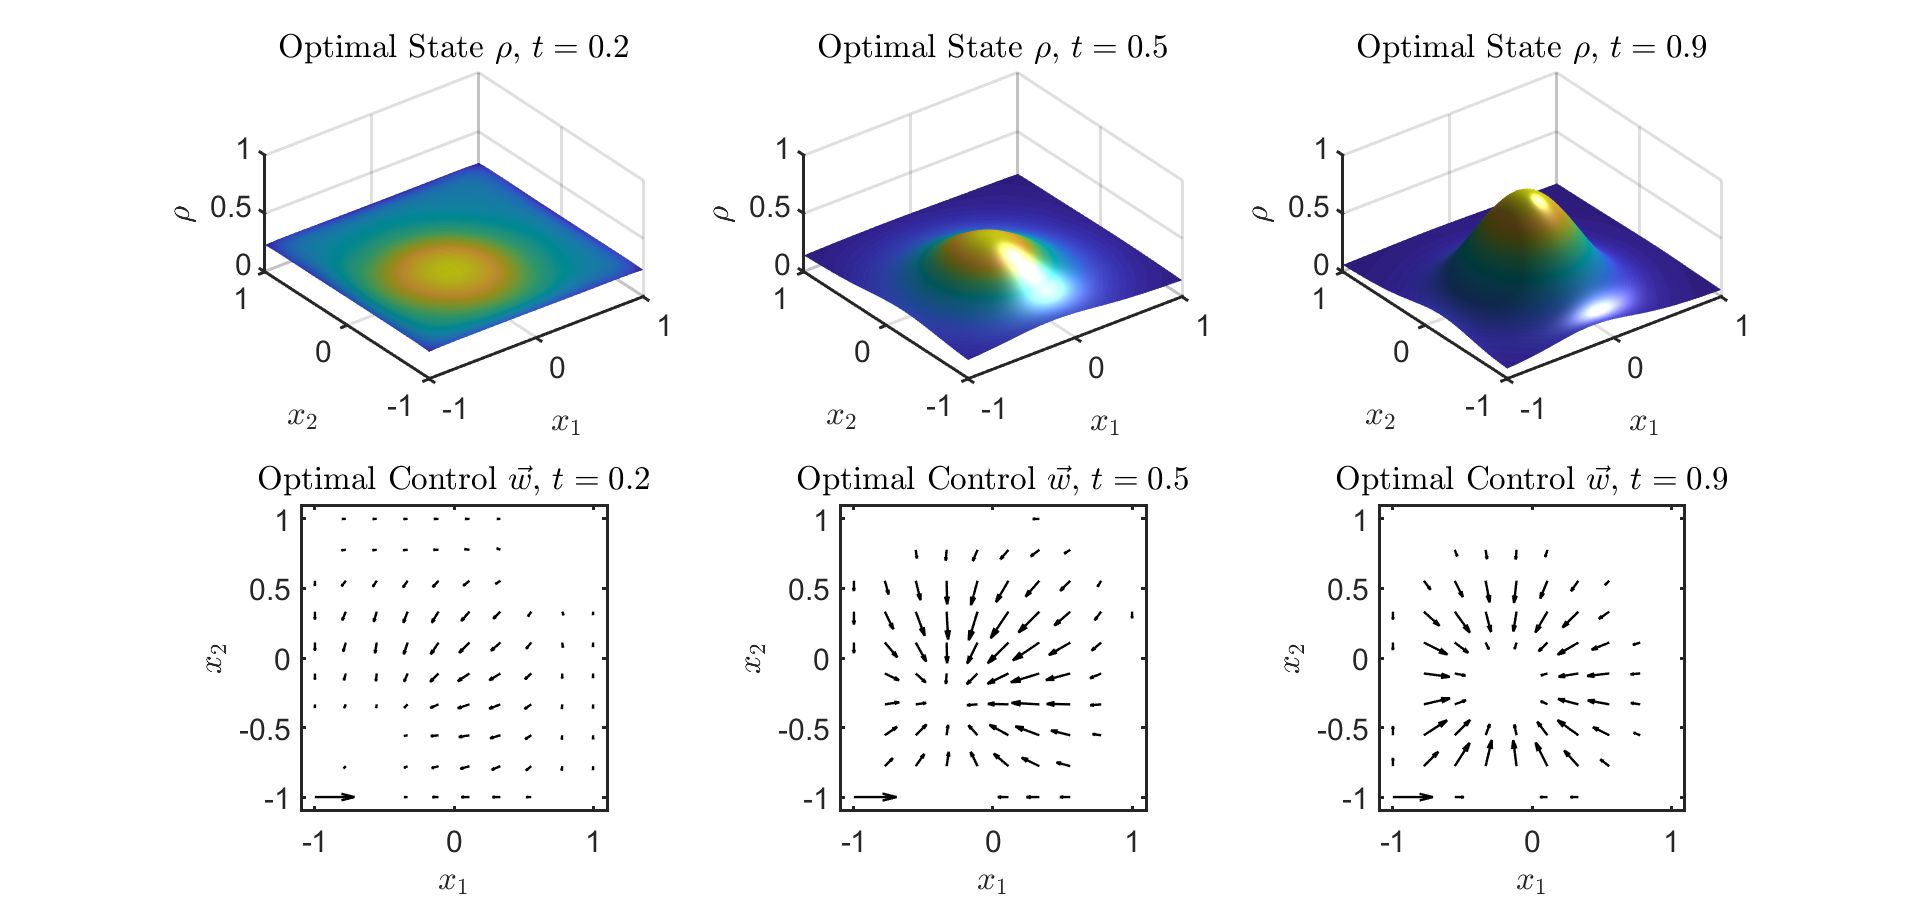
\includegraphics[scale=0.3]{Res2Ex4.png}
	\caption{2D Example 4, controlled $\rho$ and optimal control $\vec{w}$, $\beta = 10^{-3}$, $\gamma = -1$.}
	\label{rhoOpt2dEx4}
\end{figure}

Then for $\gamma = 1$, we get $J_{FW} = 0.0524$, $J_{Opt} = 0.0135$, see figures \ref{rhoHat2dEx4a} and \ref{rhoOpt2dEx4a}.
\begin{figure}[h]
	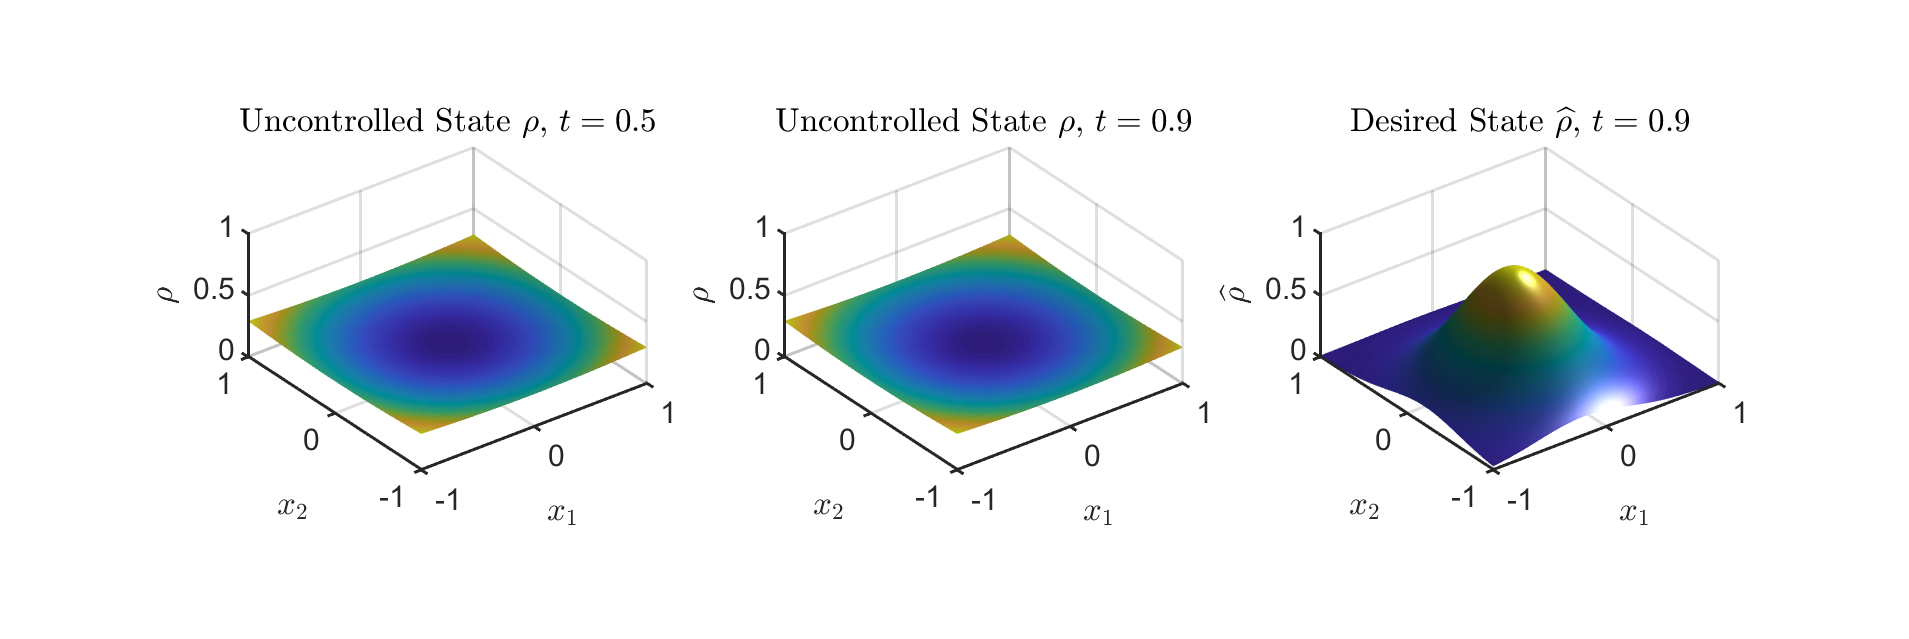
\includegraphics[scale=0.3]{Res1Ex4a.png}
	\caption{2D Example 4, uncontrolled $\rho$ and $\widehat \rho$, $\beta = 10^{-3}$, $\gamma = 1$.}
	\label{rhoHat2dEx4a}
\end{figure}
\begin{figure}[h]
	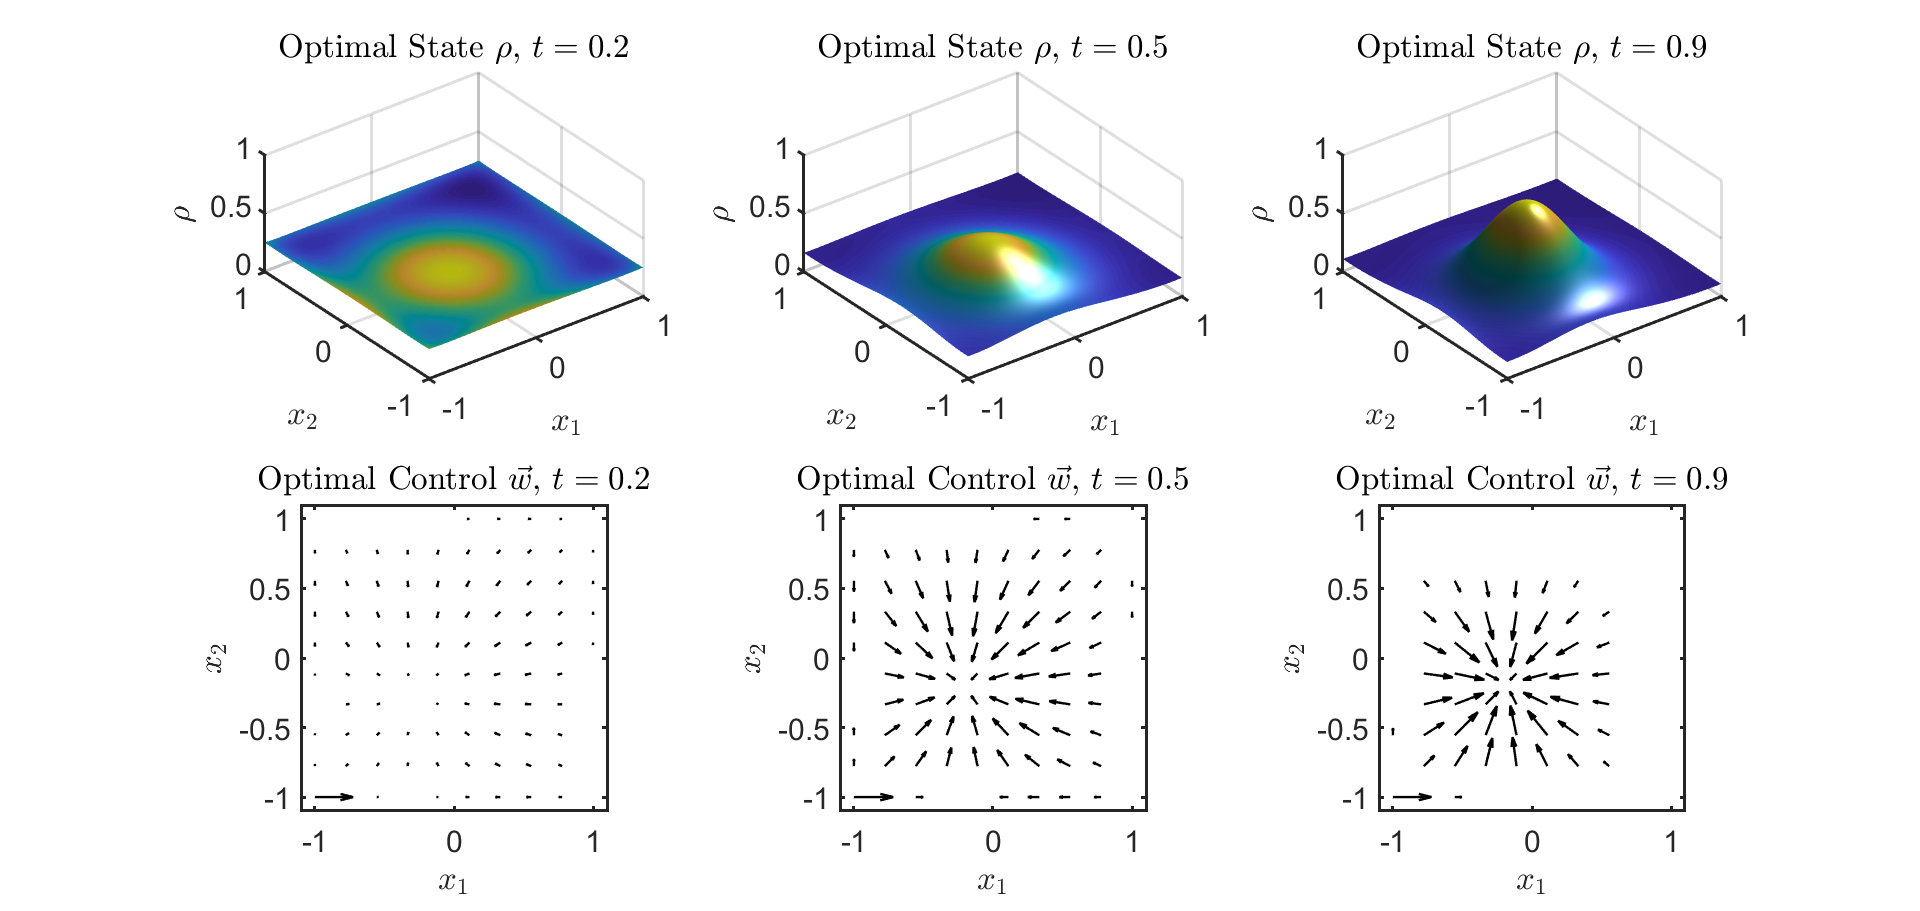
\includegraphics[scale=0.3]{Res2Ex4a.png}
	\caption{2D Example 4, controlled $\rho$ and optimal control $\vec{w}$, $\beta = 10^{-3}$, $\gamma = 1$.}
	\label{rhoOpt2dEx4a}
\end{figure}










\end{document}